\chapter{SEMI-STABLE LATTICE IN HIGHER RANK}
In this chapter, we will establish the notion of semi-stable lattice. Heuristically,
this is the lattice that achieve all the successive minima at the same time, see \cite{}.

We will provide two different definitions of semi -stable lattice: one is geometric - which follows Grayson's idea of utilizing
the canonical plot, and one is purely algebraic, which make use of the maximal standard parabolic subgroups.
The toy model will be the moduli space of 2-dimensional lattice, which is essential the upper half plane in the complex field.
At the end, we will show that the two definitions coincide.
\section{Lattices in higher rank}
For each $z$ with $\Im(z)>0$, we can attach to $z$ a lattice structure $L_z = \mathbb{Z}z \oplus \mathbb{Z}$. Roughly speaking
a lattice is a discrete  subgroup that is generated by a $k-$ basis of the $k$-space $V$.
In particular, we will only work with the real vector space $V$. Grayson works with lattice over a ring of algebraic integers, but we will restrict to
just the lattice that has the underlying structure as a $\mathbb{Z}-$ module.

\subsection{First definition of lattices}
\begin{definition}[\label = Abstract $\mathbb{Z}$-lattices]
    Let $L$ be a finitely generated $\mathbb{Z}$-module. In particular, it is a free $\mathbb{Z}$-module
    of finite rank. Suppose that $L$ is endowed with a real-valued  positive definite\footnote{The non-degenerate implicity state that rank L is the same as $dim L_\mathbb{R}$} quadratic form $Q\colon L \to \mathbb{R}$, such that the set
    \[\left\lbrace x \in L: Q(x) \le r\right\rbrace \]
    is finite for any real number $r$.
    We will call  the pair $(L,Q)$ a \textbf{abstract $\mathbb{Z}$-lattice}.
\end{definition}

An easy example is to take $L = \mathbb{Z}^n$ and choose our quadratic form to be the standard one. namely
\[\left\langle x,y \right\rangle = x \cdot y = \sum_{i=1}^n x_iy_i\]
Here the multiplication is just the usual dot product between 2 vectors. In term of matrix, this quadratic form is assigned to the
identity matrix $I_n$.

If there is no further confusion, we can just denote a Euclidean lattice by $L$, without specifying the bilinear form
$Q$. The lattice $L$ determines a full-rank lattice inside $L_\mathbb{R}$, namely, the rank
of the lattice $L$ is equal to the dimension of $L_\mathbb{R}$.

\subsection{An alternative definition of lattices}
For the sake of computation, we also usually adopt another definition of the lattice.
In particular, we view lattice as a free $\mathbb{Z}-$ module of rank $n$ that is isomorphic
to $\mathbb{R}^n$ via base changing.
\begin{definition}\label{lattice2}
    A \textit{lattice} in $\mathbb{R}^n$ is a subset $L \subset \mathbb{R}^n$ such that there exists
    a basis $b_1,\ldots,b_n$ of $\mathbb{R}^n$ such that
    \[L = \mathbb{Z}b_1\oplus \mathbb{Z}b_2\oplus \ldots \mathbb{Z}b_n\]
    If we put the vector $b_1,b_2,\ldots,b_n$ in columns, with respect to the standard basis, namely
    \[g = [b_1 | b_2 | \ldots | b_n] ,\]
    then $L = g\mathbb{Z}^n$.
\end{definition}
In the second definition, we can just identify $L$ with the standard lattice $\mathbb{Z}^n$ and the
symmetric positive definite form is $g^tg$. So an Euclidean $\mathbb{Z}$-lattice is an abstract lattice with the standard
positive definite quadratic form.
\subsection{Equivalence between two definitions of lattices}
In this subsection, we will show that every abstract $\mathbb{Z}$- lattice is isomorphic to an Euclidean $\mathbb{Z}-$ lattice.
This will be helpful in visualizing the abstract lattices, as we are just looking at concrete lattices with deformation by a linear transformation.

First we need to specify the notion of isomorphic lattices - in the first definition
\begin{definition}
    A map $f \colon (L,Q)   \to (L',Q')$  is an \textbf{isomorhism} between lattices if it is a group isomorphism and
    for all $x \in L$, we have
    \[Q(x) = Q'(f(x)) \]
\end{definition}
\begin{prop}\label{equiv-def}
    Any abstract lattice is isomorphic to a Euclidean $\mathbb{Z}-$ lattice.
\end{prop}
\begin{proof}
    Let $(L,Q)$ be an arbitrary lattice. We define a bilinear form as
    \[ \left\langle x,y \right\rangle := \dfrac{Q(x+y)-Q(x-y)}{4}\]
    We will show that this bilinear form defines an inner product over the real vector space $L_\mathbb{R} = L \otimes_\mathbb{Z} \mathbb{R}$.
    Clearly we have $\left\langle x,x \right\rangle = 4Q(x)/4 = Q(x) \ge 0$ for all $x  \in L \setminus \left\lbrace 0 \right\rbrace$.
    Now the extended bilinear form is defined as
    \begin{align*}
        \left\langle \cdot,\cdot \right\rangle  \colon L_\mathbb{R} \times L_\mathbb{R} & \to      \mathbb{R}                      \\
        (x\otimes a, y \otimes b)                                                       & \mapsto  ab\left\langle x,y\right\rangle
    \end{align*}
    It is immediate that the extended bilinear form is inner product. So we have proved that
    $L_\mathbb{R}$ is a Euclidean space containing $L$. Moreover, $L$ is embedded injectively in $L_\mathbb{R}$
    as $\mathbb{R}$ is a flat $\mathbb{Z}$ module. The condition that
    \[ \# \left\lbrace x \in L: Q(x) \le r\right\rbrace < \infty\]
    implies $L$ can be identified with a discrete in $L_\mathbb{R}$. But this implies that there exists a basis
    $\left\lbrace b_1,\ldots,b_n\right\rbrace \subset L_\mathbb{R}$  such that
    \[L = \mathbb{Z}b_1\oplus \mathbb{Z}b_2\oplus \ldots \mathbb{Z}b_n\]
    Hence we are done.\todo{fix the proof so that we use the definition 1.4.}
\end{proof}
\subsection{Covolume of a lattice}
Now that for every abstract lattice $L$ we can find an invertible matrix $g$ such that
\[ L  \cong g\mathbb{Z}^n\]

The number $n$ is called the \textbf{rank} of the lattice $L$.

Let $\left\lbrace e_1,e_2,\ldots,e_n \right\rbrace$ be an orthonormal basis of $L_\mathbb{R} \cong \mathbb{R}^n$ and
\[g = [b_1 | b_2 | \ldots | b_n] .\] The covolume of the lattice
$L$ is defined as
\begin{definition}
    The covolume of $L$ is given by the formulae
    \[\vol(L) = \left|\det(b_i\cdot e_j)\right|\]
\end{definition}
The rank and covolume are invariant numerical values of $L$, as they don't depend on the choice of basis. Indeed, two bases of a rank $n$ lattice $L$
are related by a transformation $g \in \text{GL}_n(\mathbb{Z})$. Clearly this preserves the volume and the rank as a $\mathbb{Z}-$module.


\subsection{Sublattices}
To work with semi-stable lattice $L$, we need to consider all the sublattices contained inside $L$.
\begin{definition}[\label=sublattice]
    Let $(L,Q)$ be a Euclidean $\mathbb{Z}$-lattice. We say that a $\mathbb{Z}-$submodule $M$ of
    $L$ a \textbf{sublattice} if and only if $L/M$ is torsion free.
\end{definition}
From this definition, we can prove that $M$ is a sublattice of $L$ if it satisfies one of the
following equivalent properties:
\begin{enumerate}
    \item $M$ is a summand of $L$.
    \item every basis of $M$ can be extended to a basis of $L$.
    \item The group $M$ is an intersection of $L$ with a rational subspace of $L_\mathbb{R}$.
\end{enumerate}
We refer to the \cite{} for a proof of these equivalences.
\begin{example}
    If $L = \mathbb{Z}^2$, then any sublattice of $L$ is a primitive vector $u = (a,b)$, i.e
    $\gcd(a,b)=1$. Indeed, $u=(a,b)$ is a sublattice of $\mathbb{Z}^2$ if and only if there exists a vector $v \in \mathbb{Z}^2$
    such that $L = \mathbb{Z}u \oplus \mathbb{Z}v$. With respect to the usual inner product on $\mathbb{R}^2$,
    we have
    \[1 = \vol(\mathbb{Z}^2) = \det \begin{bmatrix}
            a & b \\
            c & d
        \end{bmatrix} = ad-bc\]
    This happens if and only if $\gcd(a,b)=1$.
\end{example}
\section{Grayson's definition of semistablility}
\subsection{Grayson's definition}
In this section, we introduce the idea of Grayson in defining \textit{semi-stable} lattices.
In particular, he associates every lattices a plot and its convex hull - called \textit{ profiles}.
An easy observation is that, if $M \subset L$ is a sublattice, then the space $M_\mathbb{R} = M \otimes \mathbb{R}$
is a subspace of $L_\mathbb{R}$, equipped with the restriction of the positive definite symmetric form $Q$ of $L$, hence $M$
is also a lattice of rank not exceeding rank of $L$.
\begin{definition}[\label = slope]
    The slope of a non-zero lattice $L$ is the number
    \[\mu(L) = \dfrac{\log\vol(L)}{\dim L}\]
\end{definition}
\begin{definition}
    Suppose we have a lattice $L$. For any sublattice $M \subset L$, we assign $M$ to a point
    \[\ell(M) = \left(\dim M, \log\vol(M)\right)\]
    in the plane $\mathbb{R}^2$. The collection of all points $\ell(M)$ where $M$ ranges over
    all sublattices of $L$ is called \textbf{ the canonical plot} of the lattice $L$. By convention, we assign
    the lattice of zero rank to the origin of the plane.
\end{definition}

\begin{example}
    Add example about computing the volume of sublattices.
\end{example}
The following lemma asserts that, for each vertical axis $x =i$, there is a lowest point.
\begin{lemma}
    Given a lattice $L$ and a number $c$, there exists only a finite number of sublattices $M \subset L$ such that
    $\vol(M)<c$.
\end{lemma}
\begin{proof}
    We will prove by induction on the rank of the sublattices.
    \begin{itemize}
        \item For $r =1$, the collection of all rank $1$ sublattices of $L$ is just the set of all vectors in $L$. So we reduce
              to show that for any $c>0$, the set $B(0,c) \cap L$  has finitely many elements. But this follows immediately from the fact that
              $L$ is a discrete subset of $L_\mathbb{R}$.
        \item Assume that the lemma holds for $r >1$. Assume that
              \[M = \mathbb{Z}m_1\oplus \ldots \mathbb{Z}m_r\]
              is a sublattice of the lattices $L$ of rank $n$. Consider the wedge product $\bigwedge^r L$, then clearly
              $m_1\wedge m_2\ldots \wedge m_r$ is a vector in the lattice  $\bigwedge^r L$.
              By the previous case, there are finitely
              many vectors with bounded length inside lattice. So we only need to show that the map
              \[ M \mapsto \bigwedge^r M \]
              is finite to one, then we are done. But this is due to the observation of $\bigwedge^r M$ determines the lattice $L \cap (M \otimes \mathbb{Q})$ and the index of $M$ inside this lattice.
    \end{itemize}
    So the canonical plot is bounded below.
\end{proof}
\begin{definition}
    The boundary polygon of the convex hull of the canonical plot is called \textbf{profile} of the lattice $L$.
\end{definition}
In theory, we can compute the profile by searching for the shortest vector in each of its exterior product, but this computation
is infeasible when the dimension of the lattice grows. Since there are lattices with
arbitrarily large volume of any rank smaller than that of $L$, we add to the side the point $(0,\infty)$ and $(n,\infty)$. The sides
of the profile are therefore two vertical lines. The bottom is just the convex polygonal connecting the origin with the point
$\ell(L) = (n,\log\vol(L))$, where $n$ is the rank of $L$.
\begin{definition}\label{ss1}
    If the bottom of the profile contains only two points $(0,0)$ and $(n,\log\vol L)$, then the
    lattice $L$ is said to be \textbf{semi-stable}. Otherwise $L$ is said to be \textbf{unstable}.
\end{definition}
Below are the picture of two lattices.
\begin{figure}[hbt]
    \centering
    \begin{minipage}{.2\textwidth}
        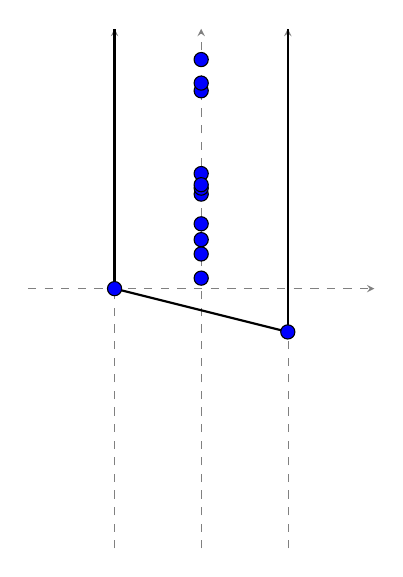
\begin{tikzpicture}[>=stealth, x=1.1cm, y=1.1cm]
            % Dashed lines (axes)
            \draw[help lines, dashed, ->] (-1,0) -- (3,0);
            \draw[help lines, dashed, ->] (0,-3) -- (0,3);
            \draw[help lines, dashed, ->] (1,-3) -- (1,3);
            \draw[help lines, dashed, ->] (2,-3) -- (2,3);
            \draw[thick] (0,0) -- (0,3);
            \draw[thick] (0,0) -- (2, -0.5);
            \draw[thick]  (2,-0.5) -- (2,3);
            \draw[thick]  (2,-0.5) -- (2,3);

            % Points (all with fill=blue and radius=0.09cm)
            \filldraw[fill=blue] (2, -0.5) circle[radius=0.09cm];
            \filldraw[fill=blue] (0, 0) circle[radius=0.09cm]; % Removed duplicate
            \filldraw[fill=blue] (1, 0.12122108098130914) circle[radius=0.09cm];
            \filldraw[fill=blue] (1, 2.28412917072110916) circle[radius=0.09cm];
            \filldraw[fill=blue] (1, 2.3729881287610001) circle[radius=0.09cm];
            \filldraw[fill=blue] (1, 0.4) circle[radius=0.09cm];
            \filldraw[fill=blue] (1, 0.5655158711807637) circle[radius=0.09cm];
            \filldraw[fill=blue] (1, 2.6445016116606668) circle[radius=0.09cm];
            \filldraw[fill=blue] (1, 0.7481703960405396) circle[radius=0.09cm];
            \filldraw[fill=blue] (1, 1.3282219276898275) circle[radius=0.09cm];
            \filldraw[fill=blue] (1, 1.0912647062501184) circle[radius=0.09cm];
            \filldraw[fill=blue] (1, 1.1603772291700336) circle[radius=0.09cm];
            \filldraw[fill=blue] (1, 1.2) circle[radius=0.09cm];
        \end{tikzpicture}~ \caption{This is a semistable lattice}
    \end{minipage} \hspace{3cm} \begin{minipage}{.2\textwidth}
        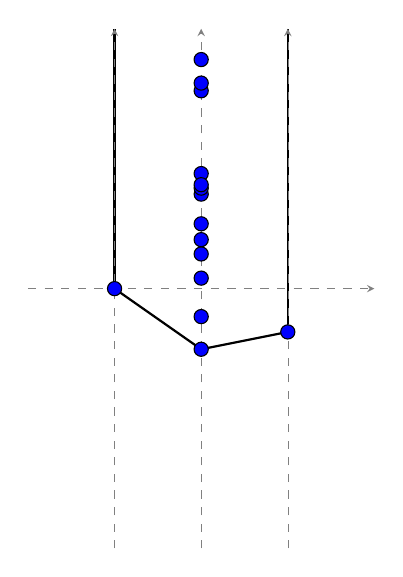
\begin{tikzpicture}[>=stealth, x=1.1cm, y=1.1cm]
            % Dashed lines (axes)
            \draw[help lines, dashed, ->] (-1,0) -- (3,0);
            \draw[thick] (0,0) -- (0,3);
            \draw[thick] (0,0) -- (1, -0.7);
            \draw[thick] (1,-0.7) -- (2,-0.5);
            \draw[thick]  (2,-0.5) -- (2,3);
            \draw[help lines, dashed, ->] (0,-3) -- (0,3);
            \draw[help lines, dashed, ->] (1,-3) -- (1,3);
            \draw[help lines, dashed, ->] (2,-3) -- (2,3);

            % Points (all with fill=blue and radius=0.09cm)
            \filldraw[fill=blue] (2, -0.5) circle[radius=0.09cm];
            \filldraw[fill=blue] (0, 0) circle[radius=0.09cm]; % Removed duplicate
            \filldraw[fill=blue] (1, -0.7) circle[radius=0.09cm];
            \filldraw[fill=blue] (1, -0.3230737092181455) circle[radius=0.09cm];
            \filldraw[fill=blue] (1, 0.12122108098130914) circle[radius=0.09cm];
            \filldraw[fill=blue] (1, 2.28412917072110916) circle[radius=0.09cm];
            \filldraw[fill=blue] (1, 2.3729881287610001) circle[radius=0.09cm];
            \filldraw[fill=blue] (1, 0.4) circle[radius=0.09cm];
            \filldraw[fill=blue] (1, 0.5655158711807637) circle[radius=0.09cm];
            \filldraw[fill=blue] (1, 2.6445016116606668) circle[radius=0.09cm];
            \filldraw[fill=blue] (1, 0.7481703960405396) circle[radius=0.09cm];
            \filldraw[fill=blue] (1, 1.3282219276898275) circle[radius=0.09cm];
            \filldraw[fill=blue] (1, 1.0912647062501184) circle[radius=0.09cm];
            \filldraw[fill=blue] (1, 1.1603772291700336) circle[radius=0.09cm];
            \filldraw[fill=blue] (1, 1.2) circle[radius=0.09cm];
        \end{tikzpicture}~
        \caption{This is an unstable lattice}
    \end{minipage}
\end{figure}
Visually, a lattice is called \textbf{semi-stable} if it satisfies the other equivalent
conditions:   If $M$ is an arbitrary sublattice of $L$ then $\mu(M) \ge \mu(L)$.
\subsection{Canonical filtration}
Given a lattice $L$ and a sublattice $M \subset L$, the quotient group $L/M$ have the structure of
a lattice. Indeed, consider the exact sequence of lattices
\[0\rightarrow M\rightarrow L\rightarrow L/M\rightarrow 0\]
By tensoring with $\mathbb{R}$ we get a short exact sequence of $\mathbb{R}$-vector subspaces
\[0\rightarrow M_\mathbb{R} \rightarrow L_\mathbb{R} \rightarrow (L/M)_\mathbb{R}\rightarrow 0,\]
which is split. Thus we have the isomorphisms
\[(L/M)_\mathbb{R} \cong L_\mathbb{R}/M_\mathbb{R} \cong M^\perp_\mathbb{R}\]
Therefore, by restriction of the inner product over $L_\mathbb{R}$ to $M^\perp_\mathbb{R}$, we clearly see that
$L/M$ also inherits an inner product. In particular, it is a lattice.
\begin{definition}
    Given a lattice $L$ containing a sublattice $M$, then $L/M$ is a lattice. We call this lattice \textbf{quotient lattice}.
\end{definition}
\begin{lemma}\label{volume-of-lattice}
    If $L$ is a lattice and $M\subset L$ is a sublattice, we have
    \[\vol(L) = \vol(M)\cdot \vol(L/M)\]
    and if $N$ is any sublattice of $L$ that satisfies $N+M=L$ then
    \[\vol(N) \ge \vol(L/M)\]
\end{lemma}
\begin{proof}
    Assume that $\{m_i\}$ is a basis for the lattice $M$ and $\{e_i\}$ be an orthonormal basis for the vector space
    $M_\mathbb{R}$. Since $M$ is a sublattice of $L$, we can extend the basis $\{m_i\}$ to get a
    basis $\{m_i\} \cup \{n_j\}$ for the lattice $L$. Similarly, we can extend  $\{e_i\}$ to get an orthonormal
    basis $\{e_i\} \cup \{f_j\}$ for the vector space $L_\mathbb{R}$. In particular, we would have
    $\left\langle m_i,f_j \right\rangle =0$ for all $i,j$.
    By definition, we have
    \begin{align*}
        vol(L) & = \det\begin{bmatrix}
                           \left\langle m_i,e_i\right\rangle  & \left\langle n_j,e_i\right\rangle \\
                           \left\langle m_i,f_J \right\rangle & \left\langle n_j,f_j\right\rangle
                       \end{bmatrix} \\
               & = \det\begin{bmatrix}
                           \left\langle m_i,e_i\right\rangle & \left\langle n_j,e_i\right\rangle \\
                           0                                 & \left\langle n_j,f_j\right\rangle
                       \end{bmatrix}  \\
               & =\vol(M)\cdot \vol(L/M)
    \end{align*}
    Hence we are done. The latter inequality follows from the fact that the volume decrease under the orthogonal projection and the observation that
    $N_\mathbb{R} \supset (L/M)_\mathbb{R}$.
\end{proof}
In the canonical plot, the import of lemma \ref{volume-of-lattice} is that the slope of the quotient lattice $L/M$ appears as
the slope of the line segment connecting the points corresponding to the sublattice $M$ and the lattice $L$. This is due to the geometry fact that
\[(\rk(M),\log(\vol(M))+ (\rk(L/M),\log\vol(L/M)))= (\rk(L),\log\vol(L))\]
\begin{figure}[ht]
    \centering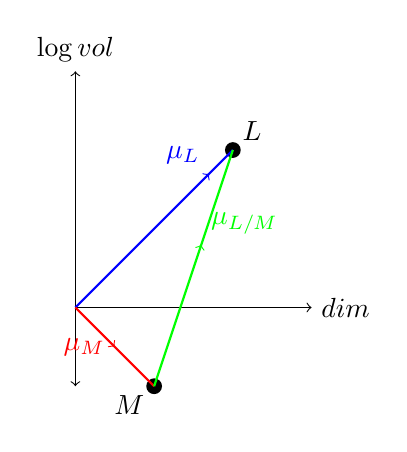
\begin{tikzpicture}
        % Draw axes
        \draw[->] (0,0) -- (3,0) node[right] {$dim$};
        \draw[->] (0,0) -- (0,3) node[above] {$\log vol$};
        \draw[->] (0,0) -- (0,-1);
        % Plot points L and M
        \fill (2,2) circle (0.1) node[above right] {$L$};
        \fill (1,-1) circle (0.1) node[below left] {$M$};

        % Draw lines from origin to L and M with colors
        \draw[thick, blue] (0,0) -- (2,2);
        \draw[thick, red] (0,0) -- (1,-1);

        % Draw line between M and L with color
        \draw[thick, green] (1,-1) -- (2,2);

        % Add mu annotations with matching colors
        \draw[->, blue] (1.5,1.5) -- (1.7,1.7) node[above left] {$\mu_L$};
        \draw[->, red] (0.3,-0.3) -- (0.5,-0.5) node[left] {$\mu_M$};
        \draw[->, green] (1.5,0.5) -- (1.6,0.8) node[above right] {$\mu_{L/M}$};
    \end{tikzpicture}
    \caption{Geometric meaning of slope in canonical plot}
\end{figure}

Given two sublattices $M_1,M_2 \subset L$, if we apply lemma \ref{volume-of-lattice} to the sublattices
$M_1/M_1\cap M_2$ and $M_2/M_1\cap M_2$ in $M_1+M_2/M_1\cap M_2$, we get
\[\vol(M_1/M_1 \cap M_2)\vol(M_2/M_1\cap M_2) \ge \vol(M_1+M_2/M_1\cap M_2)\]
or equivalently
\begin{lemma}
    \[\vol(M_1+M_2)\vol(M_1\cap M_2) \le \vol(M_1)\vol(M_2)\]
\end{lemma}
Grayson used the logarithm to express the above inequality in additive terms:
\begin{prop}\label{parallelogram-rule}
    Suppose $M_1,M_2$ are sublattices of $L$ then
    \[\log\vol(M_1)+\log(\vol(M_2)) \ge \log(\vol(M_1+M_2))+\log\vol(M_1\cap M_2)\]
\end{prop}
\begin{proof}
    It follows immediately from the fact that $\log$ is an increasing function over $(0,\infty)$.
\end{proof}
Grayson called this parallelogram rule, as the geometric meaning of  proposition \ref{parallelogram-rule} is
illustrated in the figure \ref{Grason's parallelogram rule}.
\begin{figure}[hbt!]
    \centering
    \begin{tikzpicture}
        % Coordinates
        \coordinate (A) at (0,0);
        \coordinate (B) at (4,2);
        \coordinate (C) at (6,0);
        \coordinate (D) at (2,-2);
        \coordinate (F) at (4,2.5);
        % Drawing the parallelogram
        \draw (A) -- (B) -- (C) -- (D) -- cycle;

        % Labels
        \node at (A) [above left] {$M_1 \cap M_2$};
        \node at (F) [above] {$M_1$};
        \node at (C) [above right] {$M_1 + M_2$};
        \node at (D) [below] {$M_2$};

        % Points
        \fill[cyan] (A) circle (2pt);
        \fill[cyan] (B) circle (2pt);
        \fill[cyan] (C) circle (2pt);
        \fill[cyan] (D) circle (2pt);
        \fill[cyan] (F) circle (2pt);
    \end{tikzpicture}
    \caption{\textbf{Grason's parallelogram  rule}}
    \label{Grason's parallelogram  rule}
\end{figure}
The \textbf{vertices} of the profile are the extremal/lowest points of the plot. Clearly the two points
$(0,0)$ and $(n,\log\vol(L))$ are vertices of the plot of the lattices $L$ with $\rk(L)=n$. The following lemma states the situation for other vertices
of the profile
\begin{lemma}
    Suppose that $M_\ast$ is a lattice with with the point $\ell(M_\ast)$ as a vertex of the profile. If $M$ is any other sublattice such that
    $\ell(M)$ is also a vertex of the profile, then we must have either $M \subset M_\ast$ or $M_\ast \subset M$.
\end{lemma}
\begin{figure}[H]
    \centering
    \begin{tikzpicture}
        % Coordinates
        \coordinate (A) at (0,0);
        \coordinate (B) at (4,2);
        \coordinate (C) at (6,0);
        \coordinate (D) at (2,-2);
        \coordinate (F) at (4,2.5);
        \coordinate (E) at (5,-1.5);
        \coordinate (G) at (-1,0);
        \coordinate (H) at (8,-0.5);

        % Drawing the parallelogram
        \draw (A) -- (B) -- (C) -- (D) -- cycle;

        % Labels
        \node at (A) [above left] {$M \cap M_*$};
        \node at (F) [above] {$M$};
        \node at (C) [above right] {$M + M_*$};
        \node at (D) [below] {$M_*$};
        % Points
        \fill[cyan] (A) circle (2pt);
        \fill[cyan] (B) circle (2pt);
        \fill[cyan] (C) circle (2pt);
        \fill[cyan] (D) circle (2pt);
        \fill[cyan] (F) circle (2pt);
        \fill[cyan] (E) circle (2pt);

        % draw additional lines
        \draw[gray] (G) -- (D)-- (E) -- (H);
    \end{tikzpicture}
    \caption{}
    \label{figure33}
\end{figure}
\begin{proof}
    We refer to figure \ref{figure33}. Clearly we can see that the point $\ell(M\cap M_*$) lies somewhere on the left of both
    $\ell(M)$ and $\ell(M_*)$. Similarly, the point $\ell(M+M_*)$ lies somewhere inclusively to the right of $\ell(M)$ and $\ell(M_*)$.
        By the paralellogram rule, the point $ell(M)$ will therefore be above the boundary points
    $\ell(M\cap M_*)$, $\ell(M_*)$ and $\ell(M+M_*)$. If $M$ is also a vertex of the profile, the parallelogram must degenerate. In particular we either have
    $M \cap _M*=M$, in which $M\subset M_*$, or $M+M_* = M$, in which $M_* \subset M$.
\end{proof}
An immediate consequence is that
\begin{theorem}\label{filtration}
    The vertices of the profile of a lattice $L$ are represented by unique sublattices, and they form a chain.
\end{theorem}
For a given lattice $L$, we call the chain of sublattices in theorem \ref{filtration} the \textbf{canonical filtration} of $L$. Assume that the canonical filtration for $L$
is
\[\mathcal{F}: 0 = L_0 \subset L_1 \subset L_2 \subset \cdots \subset L_{k-1} \subset L_k = L \]
then it can be seen from the diagram that
\begin{enumerate}
    \item $L_i/L_{i-1}$ is semistable for all $1 \le i \le k$.
    \item $\mu(L_i/L_{i-1}) \le \mu(L_{i+1}/L_i)$ for all $1 \le i \le k-1$.
\end{enumerate}
These two conditions is also sufficent for a chain to be a canonical filtration
\begin{theorem}\label{Grayson's criterion}
    Suppose
    \[\mathcal{F}: 0 = L_0 \subset L_1 \subset L_2 \subset \cdots \subset L_{k-1} \subset L_k = L \]
    is a chain of lattices such that $L_i/L_{i-1}$ is semistable and the slope $L_i/L_{i-1}$ is not larger than the slope of $L_{i+1}/L_i$.
    Then this chain is the canonical filtration.
\end{theorem}
\begin{figure}[ht]
    \centering
    \begin{tikzpicture}
        % Coordinates
        \coordinate (A) at (0,0);
        \coordinate (B) at (4,2);
        \coordinate (C) at (6,0);
        \coordinate (D) at (2,-2);
        \coordinate (F) at (4,2.5);
        \coordinate (E) at (5,-1.5);
        \coordinate (G) at (-1,0);
        \coordinate (H) at (8,-0.5);

        % Drawing the parallelogram
        \draw (A) -- (B) -- (C) -- (D) -- cycle;

        % Labels
        \node at (A) [above left] {$M \cap L_{i-1}$};
        \node at (F) [above] {$M$};
        \node at (C) [above right] {$M + L_{i-1}$};
        \node at (D) [below] {$L_{i-1}$};
        \node at (E) [below] {$L_i$};

        % Points
        \fill[cyan] (A) circle (2pt);
        \fill[cyan] (B) circle (2pt);
        \fill[cyan] (C) circle (2pt);
        \fill[cyan] (D) circle (2pt);
        \fill[cyan] (F) circle (2pt);
        \fill[cyan] (E) circle (2pt);

        % draw additional lines
        \draw[gray] (G) -- (D)-- (E) -- (H);
    \end{tikzpicture}
    \caption{}
    \label{figure34}
\end{figure}
\begin{proof}
    Suppose $M$ to be any other sublattice of $L$. We want to know that $\ell(M)$ lies
    above the plot $P$ of the $\ell(L_i)$. We prove by induction on the index $i$ that if $M \subset L_i$, then $\ell(M)$ lies above the
    plot $P$.
    \begin{itemize}
        \item If $i=1$ then $M\subset L_1$. Since $L_1 $is semistable, we must have $\ell(M)$ lies above the line connecting $(0,0)$ and $\ell(L_1)$. Hence $\ell(M)$ lies above the plot $P$.
        \item Suppose that $M\subset L_i$ for $i>1$. Then $M+L_{i-1} \subset L_i$ contains $L_{i-1}$. Therefore, it corresponds to the point lies above the line connecting $\ell(L_{i-1})$ and $\ell(L_i)$, thus lies above $P$.         By induction, the fact that $(M\cap L_{i-1}) \subset L_{i-1}$ implies $\ell(M\cap L_{i-1})$ lies above the plot $P$. Using the parallelogram rule, the point $\ell(M)$ must then also lie above the plot $P$
    \end{itemize}
    Thus any chain satisfies the conditions given in the theorem is a canonical filtration.
\end{proof}
\section{$\rho$- definition of semi-stability}
We are now ready to define the $\rho$-definition of semi-stable lattice. Recall that
we define the space of lattices of rank $n$ by $X_n := K \backslash \text{GL}_n(\mathbb{R})$, where $K$ is the orthogonal subgroup.
\begin{definition}[\label  = $\rho$-definition]\label{ss2}
    Let $x \in X_n$ be an arbitrary lattice, then the lattice $x$ is called \textbf{semi-stable} if and only if its degree of instability $\deg_{\text{inst}}(x)\ge 0$, where
    \[\deg_{\text{inst}}(x):= \min_{Q \in ParSt, \gamma \in \text{GL}(\mathbb{Q})/Q_i(\mathbb{Q})}\left\langle \rho_Q, H_Q(x\gamma) \right\rangle\]
\end{definition}
We first have an elementary lemma
\begin{lemma}\label{ss-equiv}
    Given $x \in X_n$, then the following are equivalent
    \begin{enumerate}
        \item $\deg_{\text{inst}}(x) \ge 0$.
        \item For every stsandard parabolic subgroup $P\subset G$ and $\omega \in \widehat{\Delta}_P$ we have \[\left\langle \omega,H_P(x\delta)\right\rangle \ge 0\] for each $\delta \in G(\mathbb{Q})/Q_i(\mathbb{Q})$.
        \item For every maximal parabolic subgroup $Q\subset G$ and $\omega \in \widehat{\Delta}_Q$ we have \[\left\langle \omega,H_Q(x\delta)\right\rangle \ge 0\] for each $\delta \in G(\mathbb{Q})/Q_i(\mathbb{Q})$.
    \end{enumerate}
\end{lemma}
\begin{proof}
    \hfill\\
    First we prove $1 \Rightarrow 3$: This follows immediately as $\rho_Q = c\omega$ for some positive number $c$ and $\omega \in \widehat{\Delta}_Q$. In particular
    \[\left\langle \omega,H_Q(x\delta) \right\rangle = \dfrac{1}{c}\left\langle \rho_Q,H_Q(x\delta) \right\rangle \ge \dfrac{1}{c}\deg_{\text{inst}}(x) \ge 0\]
    For $2 \Rightarrow 3$: We can choose a maximal standard parabolic $Q$ such that 
    $P \subset Q \subset G$. But then 
    \[\left\langle \omega,H_P(x\delta) \right\rangle =\left\langle \omega,H_Q(x\delta) \right\rangle \ge 0\]
    Finally, we have $2 \Rightarrow 1$ as $\rho_P$ is a positive linear combination of elements contained in $\widehat{\Delta}_P$.
\end{proof}
From lemma \ref{ss-equiv}, to check whether $x \in G$ is semistable, we just need to verify whether $$\left\langle \omega,H_Q(x\delta)\right\rangle \ge 0.$$
A simple observation is that - a lattice $x$ is semi - stable if for all maximal standard parabolic subgroups
$Q_i$, we have
\[\min_{\gamma \in \text{GL}_n(\mathbb{Q})/Q_i(\mathbb{Q})}\left\langle \rho_Q, H_Q(x\gamma) \right\rangle \ge 0\]
From lemma \ref{coeff-H(J)}
\[H_B = H_Q+H(B)\]
where $H_Q$ is a scalar multiple of $\lambda_i^\vee$ for $Q = Q_i$ and $H(B)$ is a linear combination of $\alpha_j^\vee$ for $ j \ne i$.
On the other hand, since $Q$ is a maximal standard parabolic subgroup of $G$,
$\rho_Q$ is proportional to $\lambda_i.$ Thus $$\left\langle \rho_Q,H(B)(x\gamma)\right\rangle =0.$$ In particular, we can replace $H_Q$ by $H_B$ in verifying the semistablility.
This implies that, if
\[ x\gamma = kan, \quad k \in K, a \in A, n \in N,\]
as in Iwasawa decomposition, then $H_B(x) = H$ where $H = \exp(a)$. In particular, if
\[a = \begin{bmatrix}
        a_1    & 0      & \ldots & 0      \\
        0      & a_2    & \ldots & 0      \\
        \vdots & \vdots & \vdots & \vdots \\
        0      & 0      & \ldots & a_n
    \end{bmatrix}\]
then
\[\left\langle \rho_{Q_i}, H_B(x\gamma) \right\rangle = \dfrac{n}{2}\log(a_1a_2\ldots a_i)\]
Thus, to check for the semi-stability of a lattice $x$, we just need to look at the
$A$-coordinate of $x\gamma$ for every $\gamma \in G(\mathbb{Q})/Q_i(\mathbb{Q})$, and verify whether the following system holds
\begin{align*}
    \begin{cases}
        a_1 \ge 1   \\
        a_1a_2\ge 1 \\
        \ldots      \\
        a_1a_2\ldots a_n \ge 1
    \end{cases}
\end{align*}
\section{Canonical pair}
Consider a pair $(P,\delta)$ of a standard parabolic subgroup $P \subsetneq G$ and $\delta \in G(\mathbb{Q})/P(\mathbb{Q})$. Such a pair is called \textbf{destabilizing} for $x$ if
\[\left\langle \rho_P, H_P(x\delta)\right\rangle = \deg_{\text{inst}}(x)\]
Such a pair is called \textbf{extremal} for $x$ if for any standard parabolic $Q \subset P$ such that
\[\left\langle \rho_Q, H_Q(x\delta)\right\rangle = \left\langle \rho_P, H_P(x\delta)\right\rangle\]
then $Q=P$.
\begin{definition}
    A pair $(P,\delta)$ that is both \textit{destabilizing} and \textit{extremal} for $x$ is called a \textbf{canonical pair} for $x$.
\end{definition}
A canonical pair for $x$, if exists, will be denoted by $\cpx:=(P,\delta)$. A priori, it is not clear whether $\cpx$ exists or not.
We will show that it is in fact equivalent to the notion of canonical filtration introduced in the previous sections, and deduce that
$\cpx$ must exist and it is unique.

We obtain the following lemma as a consequence of the definition of canonical pair
\begin{lemma}\label{canonical-pair}
    Let $x \in X_n$  and $(P,\delta)$ be a pair with $P \subsetneq G$ be standard parabolic subgroup and
    $\delta \in G(\mathbb{Q})/P(\mathbb{Q})$. Then
    \begin{enumerate}
        \item If $(P,\delta)$ is destabilizing for $x$, then $\deg_{inst}^P(x\delta) \ge 0$.
        \item If $(P,\delta) $ is extremal for $x$, then $\left\langle \alpha, H_P(x\delta)\right\rangle <0$ for any $\alpha \in \Delta_P$.
    \end{enumerate}
\end{lemma}
\begin{proof}
    For the first part, let $Q \subset P$ be any standard parabolic, then
    \[\rho_Q = \rho_P + \rho_Q^P\]
    Thus, for any $\eta \in P(\mathbb{Q})/Q(\mathbb{Q})$
    \begin{align*}
        \left\langle \rho_Q^P,H_Q(x\gamma\eta)\right\rangle & = \left\langle\rho_Q,H_Q(x\gamma\eta)\right\rangle - \left\langle\rho_P,H_P(x\gamma\eta)\right\rangle \\                                                 & = \left\langle\rho_Q,H_Q(x\gamma\eta)\right\rangle -\deg_{inst}(x) \ge 0
    \end{align*}
    For the second part, we can pick a standard parabolic $Q \subset G$ containing $P$ such that $P$ is maximal in $Q$. In particular, we have
    $\Delta^{Q}_P = \{\alpha\}$. Then
    \begin{align*}
        \left\langle\rho_P^Q,H_P(x\delta)\right\rangle & = \left\langle\rho_P,H_P(x\gamma)\right\rangle - \left\langle\rho_Q,H_Q(x\gamma\eta)\right\rangle \\
                                                       & = \deg_{inst}(x) - \left\langle\rho_Q,H_Q(x\gamma\eta)\right\rangle <0
    \end{align*}
    Since $\rho_P^Q$ and $\alpha$ are proportional by a positive number, the result follows immediately.\end{proof}
